\documentclass[conference]{IEEEtran}

% =========================================================
% PACKAGES
% =========================================================

% Restore the Times New Roman text fonts of the original build. Under XeTeX/LuaTeX
% (tectonic, or Overleaf with the compiler set to XeLaTeX) the face is used directly;
% under pdfLaTeX the class already supplies Times, so nothing is loaded and behaviour
% is unchanged. Lookup order: (1) system-installed "Times New Roman"; (2) the files
% fonts/times.ttf, timesbd.ttf, timesi.ttf, timesbi.ttf shipped inside the project
% (for Overleaf, which has no Times New Roman installed); (3) TeX Gyre Termes, a
% metric-compatible Times clone, as the last resort.
\usepackage{iftex}
\ifPDFTeX\else
  \usepackage{fontspec}
  \IfFontExistsTF{Times New Roman}
    {\setmainfont{Times New Roman}}
    {\IfFileExists{fonts/times.ttf}
      {\setmainfont{times}[Path=fonts/, Extension=.ttf,
         UprightFont=*, BoldFont=*bd, ItalicFont=*i, BoldItalicFont=*bi]}
      {\setmainfont{TeX Gyre Termes}}}
\fi

\usepackage{amsmath}
\usepackage{amssymb}
\usepackage{booktabs}
\usepackage{multirow}
\usepackage{array}
\usepackage{graphicx}
\usepackage{url}
\usepackage{hyperref}
\usepackage{float}
\usepackage{xcolor}
\usepackage{tabularx}
\usepackage{enumitem}
\usepackage{tikz}
\usetikzlibrary{arrows.meta,positioning,shapes.geometric,calc}

\hypersetup{
    colorlinks=true,
    linkcolor=black,
    citecolor=black,
    urlcolor=black
}

% ---- Tightened float and display spacing (layout only; fonts unchanged) ----
\setlength{\textfloatsep}{4pt plus 2pt minus 2pt}
\setlength{\floatsep}{4pt plus 2pt minus 2pt}
\setlength{\intextsep}{5pt plus 2pt minus 2pt}
\setlength{\dbltextfloatsep}{4pt plus 2pt minus 2pt}
\setlength{\dblfloatsep}{5pt plus 2pt minus 2pt}
\setlength{\abovecaptionskip}{1pt}
\setlength{\belowcaptionskip}{0pt}
\renewcommand{\topfraction}{0.95}
\renewcommand{\bottomfraction}{0.85}
\renewcommand{\textfraction}{0.05}
\renewcommand{\dbltopfraction}{0.95}
\renewcommand{\floatpagefraction}{0.85}
\setcounter{topnumber}{3}
\setcounter{bottomnumber}{2}
\setcounter{totalnumber}{5}
\AtBeginDocument{%
  \setlength{\abovedisplayskip}{3pt plus 2pt minus 1pt}%
  \setlength{\belowdisplayskip}{3pt plus 2pt minus 1pt}%
  \setlength{\abovedisplayshortskip}{2pt plus 1pt}%
  \setlength{\belowdisplayshortskip}{2pt plus 1pt}%
}



% =========================================================
% TITLE
% =========================================================

\title{
\textbf{EcoConnectAI: A Satellite-Driven Framework for Coastal Ecosystem Connectivity and Conservation Decision Support}
}

% =========================================================
% AUTHORS -- native IEEEtran conference author block
% =========================================================

\author{
% Author details intentionally left blank
\IEEEauthorblockN{~}
\IEEEauthorblockA{~}
}

\begin{document}

\maketitle

% =========================================================
% ABSTRACT
% =========================================================

\begin{abstract}
\bfseries
Mangroves and coastal wetlands store carbon, shelter fisheries and blunt storm surge, so knowing where they stand is a practical concern. Satellite segmentation answers that well: a weakly supervised Sentinel-1 SAR study reports about 95.56\% overall accuracy from a U-Net with an EfficientNet-B7 encoder. A map, though, never says which patches hold a landscape together, or where scarce restoration money should go. EcoConnectAI treats the habitat map as an input rather than an answer. Patches become nodes of a connectivity graph; each is deleted in turn and the resulting drop in a connectivity index becomes its criticality score; run backwards, the same machinery ranks restoration candidates by connectivity gained per unit of spending; and a rule-based layer reports the graph evidence behind every score. An interface runs these stages over prepared data for four Indian coastal landscapes, but no segmentation model has been trained and the patch geometry is synthetic, so we claim no segmentation accuracy of our own. The connectivity formulations are implemented and evaluated: in the most connected instance the patch costing the most connectivity holds only 3.8\% of habitat area and sits eleventh of eighteen by size, while the largest ranks sixth by criticality.
\end{abstract}

\begin{IEEEkeywords}
coastal ecosystem; remote sensing; habitat connectivity; satellite imagery; semantic segmentation; graph analysis; explainable AI; conservation decision support
\end{IEEEkeywords}

% =========================================================
% I. INTRODUCTION
% =========================================================

\section{Introduction}

Mangroves, seagrass meadows and tidal wetlands return far more value than their footprint suggests: they anchor fisheries, lock carbon into biomass, and blunt surge and erosion before it reaches settlements inland. Because their extent shifts under storms and bulldozers alike, planning needs habitat information that is accurate and refreshed often. Sentinel-1 SAR suits the wet tropics because radar backscatter ignores cloud and darkness, and deep learning closes the remaining gap: encoder--decoder networks hold fine detail, and weak supervision removes the need for dense hand-drawn masks.

A map, however, records \emph{where} habitat sits and is silent on \emph{how} the pieces relate. Suppose segmentation returns twenty patches and a cyclone or a new road removes one. The question is not how many hectares vanished but how badly the network was cut: a modest patch between two larger groups can fragment a landscape far more severely than a big isolated one, so area is a poor proxy for importance. Existing work covers only fragments of this: segmentation stops at the classified map; landscape ecology builds patch networks but rarely wires them to an operational pipeline; change detection reports that something happened without costing it in connectivity terms; and remote-sensing explainability explains pixels, not why a patch is load-bearing.

EcoConnectAI therefore treats mapping as the first stage of a longer pipeline: it turns a probability map into patches, wires them into a connectivity graph, scores each by a transparent criticality measure, simulates losses, states the evidence behind each score, and ranks restoration candidates by connectivity returned. Throughout we keep apart others' published results, our proposed method, what the prototype does today, and what remains unrun.

\subsection{Contributions}

\begin{enumerate}[leftmargin=*,itemsep=0pt,parsep=0pt,topsep=1pt]
    \item A habitat-mapping layer on the weakly supervised Sentinel-1 SAR methodology of the foundation study, with Sentinel-2 as a complementary input.
    \item A graph representation in which every patch is a node and every spatial relationship a weighted edge.
    \item A criticality framework pricing the connectivity lost to a patch's removal, ranking patches by structural role rather than size.
    \item A what-if module estimating the network cost of a hypothetical habitat loss.
    \item An explainability layer reporting the evidence --- area, degree, bridge position, contribution, change on removal --- behind each score.
    \item A restoration rule ranking sites by connectivity gain and, where costs exist, by gain per unit cost.
    \item An integrated architecture joining remote sensing, segmentation, graph analysis and planning in one pipeline.
    \item A working prototype of the decision-support layer over demonstration data for four Indian coastal landscapes, with the connectivity formulations implemented offline and evaluated in Section~VI.
\end{enumerate}

% =========================================================
% II. RELATED WORK
% =========================================================

\section{Related Work}

\subsection{Mangrove Mapping and Habitat Segmentation}

Sentinel-2 loses weeks to cloud in the tropical belts where mangroves grow; Sentinel-1 SAR sees through cloud at the cost of a signal less directly tied to vegetation biophysics. Our foundation study, Ghorbanian~\emph{et al.}~\cite{ghorbanian2025mangrove}, maps mangroves from time-series Sentinel-1 VV/VH imagery under weak supervision, reporting about 95.56\% overall accuracy and transferability across years --- a strong basis for our segmentation stage, but deliberately a mapping paper: no connectivity graph, no patch-level importance, no output beyond the map. Encoder--decoder networks with skip connections --- U-Net above all~\cite{ronneberger2015unet} --- dominate pixel-level habitat work, and a pretrained backbone such as EfficientNet~\cite{tan2019efficientnet} sharpens features cheaply. The foundation study fuses the two into UNB7 with weak supervision, patch-based training and test-time augmentation. Its weaknesses --- sparse stands, urban confusion --- are accuracy limits, silent on connectivity.

\subsection{Connectivity, Graphs, Change and Explanation}

Treating a landscape as a graph of patches and links is long established~\cite{urban2001landscape}, and indices such as the Probability of Connectivity (PC) and the Integral Index of Connectivity (IIC) measure what a single patch contributes to the whole~\cite{pascualhortal2006comparison,saura2007habitat}; they shape the criticality metric of Section~IV. Liu~\emph{et al.}~\cite{liu2022hybrid} build a hybrid spatiotemporal graph convolutional network over patch nodes and classify patch-level change --- fragmentation, merging, disappearance --- across long image series. This is the closest published analogue to our patch-to-graph step, but remains change \emph{detection}: it flags that a patch changed without scoring it at network level or producing a restoration output. Outside ecology, Liu and Liu~\cite{liu2025gnnresilience} review how graph neural networks quantify component importance and simulate node removal in infrastructure networks --- the nearest computational relative of our sensitivity analysis.

Change detection could trigger a what-if scenario: Naceur~\emph{et al.}~\cite{naceur2025unet} pair a spectral-index U-Net with SHAP to attribute a change to particular bands, and Yu~\emph{et al.}~\cite{yu2025changedetection} survey CNN, Siamese and transformer approaches; none price the change in connectivity terms. Klotz~\emph{et al.}~\cite{klotz2025xai} benchmark Occlusion, LIME, Grad-CAM, LRP and DeepLIFT on scene classification and expose failure modes --- baseline dependence, multi-label instability --- relevant to any attribution over habitat imagery. That work explains \emph{pixels and scenes}; why a discrete \emph{patch} matters inside a \emph{connectivity graph} is the question we take up. Finding no comparable IEEE work on AI-based restoration prioritization, we ground it in the graph-theoretic literature~\cite{urban2001landscape,pascualhortal2006comparison,saura2007habitat}. Table~\ref{tab:litcomparison} sets the reviewed work against the dimensions that matter: no study combines all of them.

\begin{table*}[!t]
\centering
\caption{Reviewed literature against the proposed framework's components (Conn.\ = connectivity, W-if = what-if, Expl.\ = explainability, Rest.\ = restoration; ``--'' = not addressed).}
\label{tab:litcomparison}
\tiny
\renewcommand{\arraystretch}{0.95}
\begin{tabularx}{\textwidth}{@{}>{\raggedright\arraybackslash}p{2.3cm}>{\raggedright\arraybackslash}p{4.2cm}>{\raggedright\arraybackslash}p{2.9cm}>{\raggedright\arraybackslash}p{3.5cm}>{\raggedright\arraybackslash}X@{}}
\toprule
\textbf{Paper / Year} & \textbf{Data and method} & \textbf{Primary task} & \textbf{Components (Conn.\,/\,W-if\,/\,Expl.\,/\,Rest.)} & \textbf{Limitation / gap} \\
\midrule
Ghorbanian \emph{et al.}, 2025~\cite{ghorbanian2025mangrove} & Sentinel-1 SAR series; weakly supervised UNB7 & Mangrove segmentation & --\,/\,--\,/\,--\,/\,-- & Habitat map only; no patch or network analysis. \\
Liu \emph{et al.}, 2022~\cite{liu2022hybrid} & Multi-temporal RS; spatiotemporal GCN & Landscape change-type detection & Partial\,/\,--\,/\,--\,/\,-- & Detects change type only; no criticality. \\
Liu \& Liu, 2025~\cite{liu2025gnnresilience} & Review of GNN node importance and resilience & Infrastructure resilience review & Yes (eng.)\,/\,Yes (rev.)\,/\,Partial\,/\,-- & Engineered domain; no remote sensing or ecology. \\
Klotz \emph{et al.}, 2025~\cite{klotz2025xai} & RS scene benchmarks; Occlusion, LIME, Grad-CAM, LRP, DeepLIFT & XAI evaluation for RS classification & --\,/\,--\,/\,Yes\,/\,-- & Explains pixels and scenes, not graph-level criticality. \\
Naceur \emph{et al.}, 2025~\cite{naceur2025unet} & Optical RS indices; spectral-index U-Net + SHAP & Change detection with explainability & --\,/\,Partial\,/\,Yes\,/\,-- & Band-level explanation; no network-level reasoning. \\
Yu \emph{et al.}, 2025~\cite{yu2025changedetection} & Bi-temporal RS; survey of CNN, Siamese, transformer CD & Change detection review & --\,/\,--\,/\,--\,/\,-- & Survey only; no connectivity or decision support. \\
\textbf{EcoConnectAI (proposed)} & Sentinel-1 SAR + Sentinel-2; segmentation, graph, sensitivity, simulation, XAI, prioritization & Connectivity-aware decision support & Yes\,/\,Yes\,/\,Yes\,/\,Yes & Prototype stage; experimental validation pending. \\
\bottomrule
\end{tabularx}
\end{table*}

% =========================================================
% III. RESEARCH GAP AND PROBLEM FORMULATION
% =========================================================

\section{Research Gap and Problem Formulation}

Fig.~\ref{fig:gap} draws the separation Table~\ref{tab:litcomparison} documents: remote sensing yields maps, graph research yields networks, explainable AI yields explanations, and no artefact is a decision. Our problem: given a habitat probability map, (i) extract discrete patches, (ii) build a graph of them and their spatial relationships, (iii) quantify each patch's contribution to connectivity, (iv) estimate the effect of losing one, (v) justify each score interpretably, and (vi) rank restoration sites by expected gain --- on top of the segmentation problem solved in~\cite{ghorbanian2025mangrove}.

\begin{figure}[!tbp]
\centering
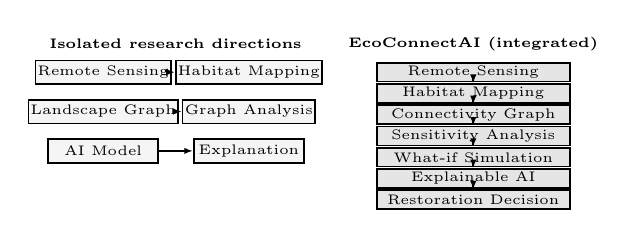
\begin{tikzpicture}[
    block/.style={rectangle, draw, semithick, fill=gray!8, minimum height=0.3cm, minimum width=1.4cm, inner sep=0.8pt, align=center, font=\tiny},
    intblock/.style={rectangle, draw, semithick, fill=gray!20, minimum height=0.24cm, minimum width=2.45cm, inner sep=0.8pt, align=center, font=\tiny},
    arrow/.style={-{Latex[length=1.1mm]}, semithick}
]
\node[block] (rs) at (0,0) {Remote Sensing};
\node[block] (hm) at (1.85,0) {Habitat Mapping};
\draw[arrow] (rs) -- (hm);
\node[block] (gr) at (0,-0.5) {Landscape Graph};
\node[block] (ga) at (1.85,-0.5) {Graph Analysis};
\draw[arrow] (gr) -- (ga);
\node[block] (ai) at (0,-1.0) {AI Model};
\node[block] (ex) at (1.85,-1.0) {Explanation};
\draw[arrow] (ai) -- (ex);
\node[font=\tiny] at (0.92,0.36) {\textbf{Isolated research directions}};

\node[intblock] (int1) at (4.7,0.0)   {Remote Sensing};
\node[intblock] (int2) at (4.7,-0.27) {Habitat Mapping};
\node[intblock] (int3) at (4.7,-0.54) {Connectivity Graph};
\node[intblock] (int4) at (4.7,-0.81) {Sensitivity Analysis};
\node[intblock] (int5) at (4.7,-1.08) {What-if Simulation};
\node[intblock] (int6) at (4.7,-1.35) {Explainable AI};
\node[intblock] (int7) at (4.7,-1.62) {Restoration Decision};
\foreach \a/\b in {int1/int2,int2/int3,int3/int4,int4/int5,int5/int6,int6/int7}{\draw[arrow] (\a) -- (\b);}
\node[font=\tiny] at (4.7,0.36) {\textbf{EcoConnectAI (integrated)}};
\end{tikzpicture}
\caption{Separate research lines versus the integrated EcoConnectAI pipeline.}
\label{fig:gap}
\end{figure}


% =========================================================
% IV. PROPOSED ECOCONNECTAI FRAMEWORK
% =========================================================

\section{Proposed EcoConnectAI Framework}

Fig.~\ref{fig:architecture} lays out the eleven-stage pipeline in three layers: satellite analysis, graph analysis, and decision support.

\begin{figure*}[!t]
\centering
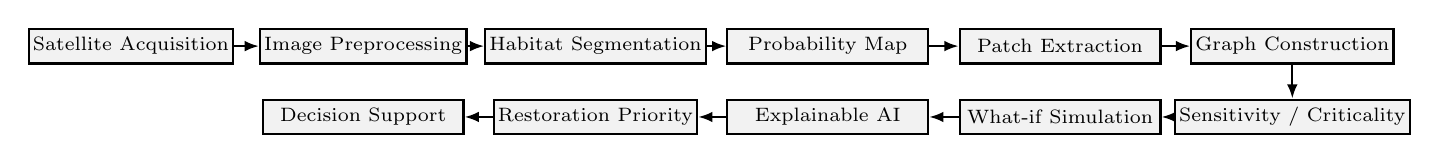
\begin{tikzpicture}[
    block/.style={rectangle, draw, thick, fill=gray!10, minimum height=0.44cm, minimum width=2.55cm, inner sep=1.5pt, align=center, font=\scriptsize},
    arrow/.style={-{Latex[length=1.8mm]}, thick}
]
\node[block] (sat)   at (0,0)     {Satellite Acquisition};
\node[block] (pre)   at (2.95,0)  {Image Preprocessing};
\node[block] (seg)   at (5.90,0)  {Habitat Segmentation};
\node[block] (prob)  at (8.85,0)  {Probability Map};
\node[block] (patch) at (11.80,0) {Patch Extraction};
\node[block] (graph) at (14.75,0) {Graph Construction};
\foreach \a/\b in {sat/pre,pre/seg,seg/prob,prob/patch,patch/graph}{\draw[arrow] (\a) -- (\b);}

\node[block] (sens)     at (14.75,-0.9) {Sensitivity / Criticality};
\node[block] (whatif)   at (11.80,-0.9) {What-if Simulation};
\node[block] (xai)      at (8.85,-0.9)  {Explainable AI};
\node[block] (restore)  at (5.90,-0.9)  {Restoration Priority};
\node[block] (decision) at (2.95,-0.9)  {Decision Support};
\draw[arrow] (graph) -- (sens);
\foreach \a/\b in {sens/whatif,whatif/xai,xai/restore,restore/decision}{\draw[arrow] (\a) -- (\b);}
\end{tikzpicture}
\caption{The EcoConnectAI pipeline, from satellite imagery to a ranked restoration plan.}
\label{fig:architecture}
\end{figure*}


\subsection{Data, Preprocessing and Segmentation}

Sentinel-1 SAR is the primary input, following the foundation methodology~\cite{ghorbanian2025mangrove}, while Sentinel-2 supplies complementary spectral indices. The two are not fused: absent a validated fusion step, SAR drives segmentation and optical indices serve elsewhere. Preprocessing covers radiometric and geometric correction, cloud masking, normalization, co-registration and tiling. Segmentation uses UNB7: an EfficientNet-B7 encoder extracting multi-level features by downsampling, a bottleneck, and a U-Net decoder upsampling back to a pixel map, with skip connections carrying encoder detail across (Fig.~\ref{fig:segmentation}). For pixel $i$ with features $X$,
\begin{equation}
P_i(c) = P(y_i = c \mid X; \theta), \qquad P_i(c) \in [0,1],
\label{eq:seg}
\end{equation}
where $y_i$ is the label of pixel $i$, $c$ a habitat class (mangrove, non-mangrove water, non-habitat), and $\theta$ the learned parameters. We keep the soft probability so patch attributes carry confidence. Weak supervision against an existing imperfect map, plus augmentation, follows the foundation study, and Eq.~\eqref{eq:seg} is what every later stage consumes. A Swin-Transformer U-Net~\cite{liu2021swin} is recorded as an alternative, its shifted-window attention giving a larger receptive field over fragmented patches; UNB7 remains the baseline pending the training set of Section~V-C.

\begin{figure}[!tbp]
\centering
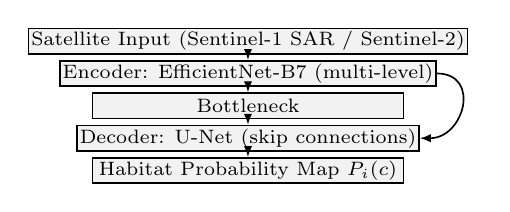
\begin{tikzpicture}[
    node distance=0.07cm,
    block/.style={rectangle, draw, semithick, fill=gray!10, minimum height=0.32cm, minimum width=3.95cm, inner sep=1pt, align=center, font=\scriptsize},
    arrow/.style={-{Latex[length=1.4mm]}, semithick}
]
\node[block] (in) {Satellite Input (Sentinel-1 SAR / Sentinel-2)};
\node[block, below=of in] (enc) {Encoder: EfficientNet-B7 (multi-level)};
\node[block, below=of enc] (bot) {Bottleneck};
\node[block, below=of bot] (dec) {Decoder: U-Net (skip connections)};
\node[block, below=of dec] (out) {Habitat Probability Map $P_i(c)$};
\draw[arrow] (in) -- (enc);
\draw[arrow] (enc) -- (bot);
\draw[arrow] (bot) -- (dec);
\draw[arrow] (dec) -- (out);
\draw[arrow] (enc.east) to[out=0,in=0,looseness=1.7] (dec.east);
\end{tikzpicture}
\caption{Segmentation architecture inherited from the foundation study (UNB7).}
\label{fig:segmentation}
\end{figure}

\subsection{Patch Extraction and Graph Construction}

Contiguous above-threshold regions are grouped into connected components, each a patch described by
\begin{equation}
\text{Patch}_i = \{A_i, (x_i, y_i), C_i, H_i\},
\label{eq:patch}
\end{equation}
with $A_i$ the area, $(x_i, y_i)$ the centroid, $C_i \in [0,1]$ a confidence from the mean probability inside the patch, and $H_i$ the habitat class --- the interface between segmentation and the graph. We fix the class-probability threshold at $0.5$ and drop components below a $2$~ha minimum mapping unit; both are uncalibrated parameters to revisit once a model is trained. Patches form a graph
\begin{equation}
G = (V, E),
\label{eq:graph}
\end{equation}
with $V$ the patches and $E$ their connectivity relationships (Fig.~\ref{fig:patchgraph}). In the simplest form an edge exists when separation stays within a threshold $\tau$,
\begin{equation}
A_{ij} =
\begin{cases}
1, & d_{ij} \leq \tau \\
0, & \text{otherwise},
\end{cases}
\label{eq:binary_edge}
\end{equation}
where $d_{ij}$ is the distance between centroids or nearest boundaries. A binary edge discards how strongly two patches are tied, so we propose a weighted extension,
\begin{equation}
w_{ij} = f(d_{ij}, \; \text{habitat\_similarity}_{ij}, \; C_i, C_j),
\label{eq:weighted_edge}
\end{equation}
with $f(\cdot)$ a proposed scoring function --- not an ecological law --- falling with distance and rising with similarity and confidence, so Section~IV-C can tell a short strong link from a marginal one. The instantiation we adopt couples exponential decay to a quality term,
\begin{equation}
w_{ij} = q_{ij} \, \exp\!\left(-\frac{d_{ij}}{\tau}\right), \qquad q_{ij} = \sqrt{q_i q_j},
\label{eq:decay}
\end{equation}
where $q_i \in [0,1]$ is patch quality, from confidence $C_i$ and habitat condition, and $q_{ij}$ their geometric mean. Edges are restricted to the $k = 3$ nearest neighbours with $d_{ij} \leq \tau$, keeping the graph sparse. The threshold $\tau$ is species-relevant, hence a per-deployment calibration parameter: any reported $\tau$ must name the species it stands for.

\begin{figure}[!tbp]
\centering
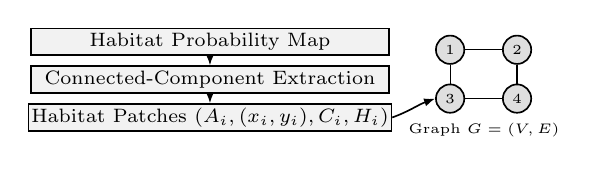
\begin{tikzpicture}[
    block/.style={rectangle, draw, semithick, fill=gray!10, minimum height=0.34cm, minimum width=4.55cm, inner sep=1pt, align=center, font=\scriptsize},
    arrow/.style={-{Latex[length=1.4mm]}, semithick},
    patchnode/.style={circle, draw, semithick, fill=gray!25, minimum size=0.36cm, inner sep=0pt, font=\tiny}
]
\node[block] (map)     at (0,0)     {Habitat Probability Map};
\node[block] (comp)    at (0,-0.48) {Connected-Component Extraction};
\node[block] (patches) at (0,-0.96) {Habitat Patches ($A_i,(x_i,y_i),C_i,H_i$)};
\draw[arrow] (map) -- (comp);
\draw[arrow] (comp) -- (patches);

\node[patchnode] (n1) at (3.05,-0.10) {1};
\node[patchnode] (n2) at (3.90,-0.10) {2};
\node[patchnode] (n3) at (3.05,-0.72) {3};
\node[patchnode] (n4) at (3.90,-0.72) {4};
\draw (n1) -- (n2); \draw (n1) -- (n3); \draw (n2) -- (n4); \draw (n3) -- (n4);
\draw[arrow] (patches.east) to[out=20,in=200] (n3.west);
\node[font=\tiny] at (3.48,-1.12) {Graph $G=(V,E)$};
\end{tikzpicture}
\caption{Habitat probability map to patches to connectivity graph.}
\label{fig:patchgraph}
\end{figure}

\subsection{Connectivity Sensitivity and Criticality}

Over $G$ we compute a scalar connectivity measure $C(G)$ --- as plain as the largest connected component, or an index such as PC or IIC~\cite{pascualhortal2006comparison,saura2007habitat}. We fix no single choice; the analysis holds for \emph{any} such measure. The prototype's index is a composite normalized to $[0,100]$,
\begin{equation}
C(G) = 100 \sum_{k=1}^{5} \omega_k \, n_k(G), \qquad \sum_{k=1}^{5} \omega_k = 1,
\label{eq:composite}
\end{equation}
where $n_k(G) \in [0,1]$ is the $k$-th normalized component --- structural and functional connectivity, habitat quality, patch redundancy, protection coverage --- weighted at $0.30$, $0.28$, $0.22$, $0.12$ and $0.08$, the first two from IIC and PC~\cite{pascualhortal2006comparison,saura2007habitat}. That weighting is our design choice, unvalidated against field data, and stated so results from it can be challenged. Removing patch $i$ with its incident edges costs
\begin{equation}
\Delta C_i = C(G) - C(G - v_i),
\label{eq:deltac}
\end{equation}
where $G - v_i$ is the graph after deleting node $v_i$; a large $\Delta C_i$ marks a patch carrying more connectivity than its size suggests. Normalizing for comparability gives the criticality score
\begin{equation}
S_i = \frac{\Delta C_i}{C(G)} = \frac{C(G) - C(G-v_i)}{C(G)},
\label{eq:criticality}
\end{equation}
writing $C(G)$ as $C_{\text{base}}$ and $C(G - v_i)$ as $C_{-i}$. Higher $S_i$ means greater exposure to losing that patch; the formulation is consistent with, though not identical to, PC and IIC~\cite{pascualhortal2006comparison,saura2007habitat}. The procedure: compute $C(G)$; for each $i$, delete $v_i$ and its edges; recompute; obtain $S_i$; sort descending.

\subsection{What-if Simulation}

The what-if module points the same mechanism at one scenario the user picks. In the running example, twenty patches include $P_7$, sitting between several loosely joined groups. Baseline connectivity is $C_{\text{base}}$; deleting $P_7$ and rebuilding gives $C_{\text{after}}$, so the loss is
\begin{equation}
\Delta C = C_{\text{base}} - C_{\text{after}}.
\label{eq:whatif}
\end{equation}
Eq.~\eqref{eq:whatif} is the single-scenario case of Eq.~\eqref{eq:deltac}. Fig.~\ref{fig:whatif} draws it: $P_7$ may hold a sliver of area, yet its removal severs an otherwise linked chain, making $\Delta C$ out of all proportion to the hectares lost --- where area-based prioritization understates a bridge patch. These values are illustrative.

\begin{figure}[!tbp]
\centering
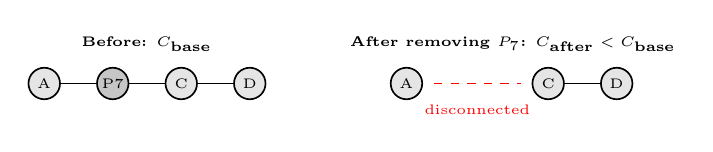
\begin{tikzpicture}[
    patchnode/.style={circle, draw, semithick, fill=gray!20, minimum size=0.4cm, inner sep=0pt, font=\tiny},
    bridgenode/.style={circle, draw, semithick, fill=gray!45, minimum size=0.4cm, inner sep=0pt, font=\tiny},
    lbl/.style={font=\tiny}
]
\node[lbl] at (1.3,0.5) {\textbf{Before: $C_{\text{base}}$}};
\node[patchnode] (A) at (0,0) {A};
\node[bridgenode] (B) at (0.87,0) {P7};
\node[patchnode] (C) at (1.74,0) {C};
\node[patchnode] (D) at (2.61,0) {D};
\draw (A) -- (B); \draw (B) -- (C); \draw (C) -- (D);

\node[lbl] at (5.95,0.5) {\textbf{After removing $P_7$: $C_{\text{after}} < C_{\text{base}}$}};
\node[patchnode] (A2) at (4.6,0) {A};
\node[patchnode] (C2) at (6.4,0) {C};
\node[patchnode] (D2) at (7.27,0) {D};
\draw (C2) -- (D2);
\draw[dashed,red] (4.95,0) -- (6.05,0);
\node[lbl,red] at (5.5,-0.33) {disconnected};
\end{tikzpicture}
\caption{Illustrative what-if scenario: removing bridge patch P7 strands A.}
\label{fig:whatif}
\end{figure}

\subsection{Explainable AI}

Instead of a bare score, the explainability layer reports the evidence behind it: area $A_i$; degree in $G$; whether the patch is a bridge or cut vertex; neighbour distances; confidence $C_i$; local contribution before removal; and the measured $\Delta C_i$. A sentence follows --- e.g.\ \emph{``critical because it joins three otherwise weakly connected regions, holds degree 3, and its removal drops connectivity by $\Delta C_i$''} (Fig.~\ref{fig:xai}). Where Grad-CAM, SHAP or LIME is applied to the segmentation model rather than the graph score, it should follow~\cite{klotz2025xai,naceur2025unet}. The graph-level explanation is rule-based and needs no post-hoc attribution.

\begin{figure}[!tbp]
\centering
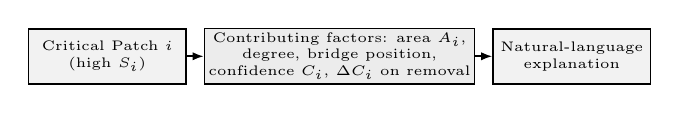
\begin{tikzpicture}[
    block/.style={rectangle, draw, semithick, fill=gray!10, minimum height=0.7cm, minimum width=2.0cm, inner sep=1.5pt, align=center, font=\tiny},
    wideblock/.style={rectangle, draw, semithick, fill=gray!15, minimum height=0.7cm, minimum width=3.4cm, inner sep=1.5pt, align=center, font=\tiny},
    arrow/.style={-{Latex[length=1.4mm]}, semithick}
]
\node[block] (patch) at (0,0) {Critical Patch $i$\\(high $S_i$)};
\node[wideblock] (factors) at (2.95,0) {Contributing factors: area $A_i$,\\degree, bridge position,\\confidence $C_i$, $\Delta C_i$ on removal};
\node[block] (text) at (5.9,0) {Natural-language\\explanation};
\draw[arrow] (patch) -- (factors);
\draw[arrow] (factors) -- (text);
\end{tikzpicture}
\caption{Explainability: the graph quantities that produced a patch's score.}
\label{fig:xai}
\end{figure}

\subsection{Restoration Prioritization and Output}

Restoration prioritization inverts the sensitivity analysis: it measures the connectivity won by adding a patch. A candidate $v_i$ is inserted into $G$, connectivity recomputed, and the gain taken as
\begin{equation}
R_i = C(G + v_i) - C(G).
\label{eq:gain}
\end{equation}
Where an intervention cost is known, the cost-aware score is
\begin{equation}
\text{Priority}_i = \frac{R_i}{\text{Cost}_i}.
\label{eq:priority}
\end{equation}
This stops the ranking collapsing into ``restore the biggest available site'' and rewards the candidate returning most connectivity per unit of resource (Fig.~\ref{fig:restoration}). Without cost data, $\text{Priority}_i$ reduces to $R_i$. The final stage gathers map, graph, criticality ranking, what-if outcomes, explanations and restoration ranking into a report informing, not replacing, ecological judgement.

\begin{figure}[!tbp]
\centering
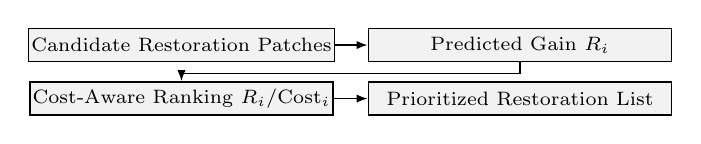
\begin{tikzpicture}[
    block/.style={rectangle, draw, semithick, fill=gray!10, minimum height=0.42cm, minimum width=3.85cm, inner sep=1pt, align=center, font=\scriptsize},
    arrow/.style={-{Latex[length=1.4mm]}, semithick}
]
\node[block] (cand) at (0,0)        {Candidate Restoration Patches};
\node[block] (gain) at (4.3,0)      {Predicted Gain $R_i$};
\node[block] (cost) at (0,-0.68)    {Cost-Aware Ranking $R_i / \text{Cost}_i$};
\node[block] (rank) at (4.3,-0.68)  {Prioritized Restoration List};
\draw[arrow] (cand) -- (gain);
\draw[arrow] (gain.south) -- ++(0,-0.14) -| (cost.north);
\draw[arrow] (cost) -- (rank);
\end{tikzpicture}
\caption{Restoration prioritization: gain ranked, adjusted for cost where available.}
\label{fig:restoration}
\end{figure}

% =========================================================
% V. EXPERIMENTAL SETUP
% =========================================================

\section{Implementation Status and Experimental Setup}

\subsection{Prototype Implementation Status}

The decision-support layer is a client-side web application (Next.js, React, TypeScript, with Leaflet, React Flow and Recharts). There is no backend, database or ML runtime: every habitat mask, patch attribute, graph, sensitivity surface and scenario projection comes from prepared datasets through one typed data-access module, so trained-model output can later replace them without touching the analysis or interface code. Table~\ref{tab:implstatus} maps each stage of Fig.~\ref{fig:architecture} to its status. Those datasets are synthetic --- a deterministic generator produced them so the interface could exercise the workflow consistently --- so they are not measurements. Only the metadata in Table~\ref{tab:studyareas} is real, and no number the prototype displays is reported as a result.

\begin{table}[!tbp]
\centering
\caption{Implementation status of each stage of Fig.~\ref{fig:architecture}.}
\label{tab:implstatus}
\tiny
\renewcommand{\arraystretch}{0.95}
\begin{tabularx}{\columnwidth}{@{}p{1.55cm}>{\raggedright\arraybackslash}X@{}}
\toprule
\textbf{Stage} & \textbf{Status in the current prototype} \\
\midrule
Acquisition & Scene-selection interface; no imagery retrieved or processed. \\
Preprocessing & Not implemented; a staged progress display only. \\
Segmentation & Not implemented. No model trained, no inference run. \\
Probability map & Prepared: per-class area, coverage share, mean confidence. \\
Patch extraction & Prepared: 16--20 patches with area, quality, confidence, degree, bridge score. \\
Connectivity graph & Prepared: 30--39 edges; rendered, queried and traversed interactively. \\
Sensitivity / criticality & Interface: prepared leave-one-out surface of 426--508 grid cells, four bands. Offline: $S_i$ computed exactly per Eq.~\eqref{eq:criticality} over all patches of all four landscapes. \\
What-if simulation & Removal, severed-edge and isolation detection. The interface's drop is heuristic; offline recomputes $C(G)$ exactly. \\
Explainable AI & Rule-based graph explanation of Section~IV-E; no post-hoc attribution, as there is no model to attribute. \\
Restoration & Budget-constrained selection ranked per Eq.~\eqref{eq:priority}; offline, each $R_i$ recomputed by node addition. \\
Decision output & Implemented: report composition and export. \\
\bottomrule
\end{tabularx}
\end{table}

\subsection{Study Areas and Satellite Configuration}

The system is configured for four Indian coastal landscapes, chosen for protection status, habitat mix (mangrove, seagrass, salt marsh, mudflat, coral, estuarine channel) and their distinct pressures; Table~\ref{tab:studyareas} lists them with sensor and ground sample distance. This does not displace the Sentinel-1 SAR baseline of Section~IV-A.

\begin{table}[!tbp]
\centering
\caption{Coastal landscapes and satellite configurations; footprint is the configured scene extent.}
\label{tab:studyareas}
\scriptsize
\renewcommand{\arraystretch}{0.95}
\begin{tabularx}{\columnwidth}{@{}>{\raggedright\arraybackslash}X>{\raggedright\arraybackslash}p{1.5cm}cc@{}}
\toprule
\textbf{Landscape} & \textbf{Sensor} & \textbf{GSD} & \textbf{Footprint} \\
\midrule
Vembanad--Kol, Kerala (Ramsar) & Sentinel-2 L2A & 10\,m & 486\,km$^2$ \\
Sundarbans W.\ Delta, W.B.\ (UNESCO) & Sentinel-2 L2A & 10\,m & 1284\,km$^2$ \\
Gulf of Mannar reefs, T.N.\ (Marine NP) & Landsat-9 OLI-2 & 30\,m & 826\,km$^2$ \\
Bhitarkanika, Odisha (Ramsar / NP) & Sentinel-2 L2A & 10\,m & 672\,km$^2$ \\
\bottomrule
\end{tabularx}
\end{table}

\subsection{Experimental Configuration}

Table~\ref{tab:expsetup} records the configuration behind Section~VI with the fixed segmentation settings. The two software rows are separate on purpose: the first is what the implemented components use, the second the stack expected for the unwritten segmentation stage. Four quantities stay unfixed until that experiment runs --- acquisition window, scene count, data split and hardware.

\begin{table}[!tbp]
\centering
\caption{Experimental configuration; the analysis parameters are those under which every result of Section~VI was computed.}
\label{tab:expsetup}
\tiny
\renewcommand{\arraystretch}{0.95}
\begin{tabularx}{\columnwidth}{@{}p{1.75cm}>{\raggedright\arraybackslash}X@{}}
\toprule
\textbf{Item} & \textbf{Value} \\
\midrule
Study areas & Four Indian coastal landscapes (Table~\ref{tab:studyareas}) \\
Satellite source & Sentinel-1 SAR (VV, VH)~\cite{ghorbanian2025mangrove}; Sentinel-2 MSI L2A at 10\,m, Landsat-9 OLI-2 at 30\,m for indices \\
Segmentation & UNB7~\cite{ghorbanian2025mangrove}, weakly supervised against an existing ecosystem map; Swin-Transformer U-Net~\cite{liu2021swin} an alternative \\
Training tiles & $\approx$14\,000 labelled $512 \times 512$ tiles; sources: Forest Survey of India atlas, national wetland inventory, Ramsar boundaries \\
Patch extraction & Class-probability threshold $0.5$; minimum mapping unit $2$\,ha \\
Graph construction & $k = 3$ neighbours with $d_{ij} \leq \tau$; weight per Eq.~\eqref{eq:decay}; $\tau = 5$\,km, with $\tau \in \{3,5,8\}$\,km in Section~VI-F \\
Connectivity measure & $C(G) = \mathrm{IIC}$~\cite{pascualhortal2006comparison}, PC and ECA alongside; interface score Eq.~\eqref{eq:composite}, weights $0.30/0.28/0.22/0.12/0.08$ \\
Sensitivity grid & 100\,m analysis grid, four sensitivity bands \\
Criticality / restoration & $S_i$ per Eq.~\eqref{eq:criticality} by exact node removal; $R_i$ per Eq.~\eqref{eq:gain} by node addition; Priority$_i$ per Eq.~\eqref{eq:priority} \\
Software (built) & TypeScript, React, Next.js, Leaflet, React Flow, Recharts; Python 3, standard library only (Section~VI) \\
Software (planned) & PyTorch; Rasterio; GeoPandas; OpenCV (segmentation, not yet written) \\
\bottomrule
\end{tabularx}
\end{table}

% =========================================================
% VI. RESULTS AND DISCUSSION
% =========================================================

\section{Results and Discussion}

\subsection{Scope of the Reported Results}

Section~VI-B reproduces accuracy published by the foundation study, which our segmentation stage inherits and which is \emph{not} a measurement of this work; Sections~VI-C--VI-F report results from our implementation of Eqs.~\eqref{eq:binary_edge}--\eqref{eq:priority}. Their habitat geometry is the synthetic data of Section~V-A, so they validate the method on defined landscape instances rather than measuring any real ecosystem; patches carry indices (P01--P20). The analysis is genuinely computed and reproducible: written in Python using the standard library alone --- no graph package, so every index comes from its definition --- and run over all four landscapes, so each value in Tables~\ref{tab:connbaseline}--\ref{tab:restoreresults} regenerates from the accompanying script. $C(G)$ is evaluated as IIC~\cite{pascualhortal2006comparison} rather than Eq.~\eqref{eq:composite}, so the criticality values owe nothing to our weighting; PC and Equivalent Connected Area (ECA)~\cite{saura2007habitat} are reported alongside. The graph uses $k = 3$, $\tau = 5$~km, and for PC $p_{ij} = \exp(-\alpha d_{ij})$ with $\alpha$ set so $p = 0.5$ at $d = \tau$.

\subsection{Segmentation Baseline Inherited from the Foundation Study}

Our segmentation stage adopts UNB7 unmodified and inherits its published accuracy; Table~\ref{tab:segbaseline} reproduces those figures with the random-forest comparison from the same study~\cite{ghorbanian2025mangrove}. We have trained no model and claim no independent accuracy; establishing one over the landscapes of Table~\ref{tab:studyareas} is the immediate next step.

\begin{table}[!tbp]
\centering
\caption{Segmentation accuracy \emph{reported by the foundation study}~\cite{ghorbanian2025mangrove} for the adopted UNB7 architecture --- their measurements, not results of this work.}
\label{tab:segbaseline}
\scriptsize
\renewcommand{\arraystretch}{0.95}
\begin{tabular}{@{}lcc@{}}
\toprule
\textbf{Metric} & \textbf{UNB7 (adopted)} & \textbf{RF baseline} \\
\midrule
Overall accuracy & 95.56\% & 77.35\% \\
Kappa coefficient & 0.94 & 0.74 \\
F1-score & 0.95 & --- \\
Mean producer's accuracy & 95.37\% & --- \\
Mean user's accuracy & 95.90\% & --- \\
\bottomrule
\end{tabular}
\end{table}

\subsection{Landscape Connectivity Baseline}

Across all four landscapes (Table~\ref{tab:connbaseline}) equivalent connected area lands between $53.7\%$ and $59.6\%$ of mapped habitat area: each fragmented network delivers the connectivity of a single patch roughly half its extent, and closing that shortfall is what a restoration programme is for. Kerala is the most connected instance ($18$ links over $18$ patches, three components); Sundarbans is the most fragmented at $\tau = 5$~km, breaking into $12$ components over $20$ patches --- the wider patch spacing of a delta at a fixed threshold, not a property of the ecosystem, and one reason a single $\tau$ across landscapes of differing extent is flagged in Section~VII.

\begin{table}[!tbp]
\centering
\caption{Baseline connectivity; graph per Section~IV-B, $k=3$, $\tau = 5$~km. $|V|$, $|E|$, comp.: patch, link, component counts.}
\label{tab:connbaseline}
\scriptsize
\setlength{\tabcolsep}{3.5pt}
\renewcommand{\arraystretch}{0.95}
\begin{tabular}{@{}lccccccc@{}}
\toprule
\textbf{Landscape} & $|V|$ & $|E|$ & \textbf{comp.} & \textbf{IIC} & \textbf{PC} & \textbf{ECA} & \textbf{ECA} \\
 & & & & $\times 10^{3}$ & $\times 10^{3}$ & \textbf{(ha)} & \textbf{\%} \\
\midrule
Kerala coast    & 18 & 18 & 3  & 5.38 & 7.28 & 4147 & 59.6 \\
Sundarbans      & 20 & 10 & 12 & 0.55 & 1.54 & 5045 & 53.7 \\
Gulf of Mannar  & 17 & 12 & 9  & 0.81 & 2.05 & 3741 & 55.1 \\
Odisha coast    & 16 & 10 & 8  & 1.91 & 4.40 & 4460 & 54.7 \\
\bottomrule
\end{tabular}
\end{table}

\subsection{Patch Criticality}

Table~\ref{tab:sensresults} gives the criticality ranking for Kerala, where network position and area part company most sharply. The central result sits in rows one and six. P16 holds $3.8\%$ of mapped habitat and ranks $11$th of $18$ by area, yet losing it costs more connectivity than losing anything else ($S_{16} = 0.408$, a $40.8\%$ cut in IIC) and splits the network from three components into five. The largest patch, P14 ($820.6$~ha, $11.8\%$, first by area), ranks only sixth ($S_{14} = 0.245$), leaving the component count at three. Structural position, not size, decides what losing a patch costs. The most critical patch was not the largest in three of four instances, ranking $11$th of $18$ (Kerala), $2$nd of $20$ (Sundarbans) and $3$rd of $16$ (Odisha) by area; only in the Gulf of Mannar, where one shelf dominates area and anchors the network, did the rankings agree.

\begin{table}[!tbp]
\centering
\caption{Patch criticality for Kerala, ranked by $S_i$ (Eq.~\eqref{eq:criticality}), $C(G) = \mathrm{IIC}$. Comp.\ = components after removal (baseline 3); Area rk.\ = rank by area. Top nine of 18.}
\label{tab:sensresults}
\scriptsize
\setlength{\tabcolsep}{3pt}
\renewcommand{\arraystretch}{0.95}
\begin{tabular}{@{}ccccccccc@{}}
\toprule
\textbf{Rank} & \textbf{Patch} & \textbf{Area} & \textbf{Area} & \textbf{Deg.} & $\Delta C_i$ & $S_i$ & \textbf{Comp.} & \textbf{Area} \\
 & & \textbf{(ha)} & \textbf{\%} & & $\times 10^{3}$ & & & \textbf{rk.} \\
\midrule
1 & P16 & 263.0 & 3.8  & 3 & 2.192 & 0.408 & 5 & 11 \\
2 & P15 & 684.3 & 9.8  & 3 & 2.113 & 0.393 & 4 & 2 \\
3 & P02 & 211.6 & 3.0  & 3 & 1.859 & 0.346 & 5 & 12 \\
4 & P03 & 159.6 & 2.3  & 3 & 1.381 & 0.257 & 4 & 14 \\
5 & P05 & 657.2 & 9.4  & 3 & 1.334 & 0.248 & 4 & 3 \\
6 & P14 & 820.6 & 11.8 & 3 & 1.317 & 0.245 & 3 & 1 \\
7 & P17 & 355.2 & 5.1  & 2 & 1.042 & 0.194 & 4 & 9 \\
8 & P12 & 610.1 & 8.8  & 2 & 0.854 & 0.159 & 3 & 4 \\
9 & P18 & 590.3 & 8.5  & 1 & 0.747 & 0.139 & 3 & 6 \\
\bottomrule
\end{tabular}
\end{table}

\subsection{Restoration Prioritization}

Table~\ref{tab:restoreresults} gives the restoration ranking for Kerala. Each candidate is added to the graph, its links form under the same $k$ and $\tau$ rule, and connectivity is recomputed for $R_i$ per Eq.~\eqref{eq:gain}. Costs are indicative planning values, not surveyed estimates, so the ranking demonstrates the mechanism of Eq.~\eqref{eq:priority} rather than recommending funding. It separates two questions a planner must keep apart: C5 buys the largest raw gain ($+3.50\%$), but at INR~807 lakh drops to fifth once cost enters, while C1 ($+2.73\%$ at INR~466 lakh) takes first. C8 fails on both, forming one link for $+0.07\%$. Ranking by restored area would not reproduce this order.

\begin{table}[!tbp]
\centering
\caption{Restoration prioritization for Kerala. $R_i$: gain of Eq.~\eqref{eq:gain}, \% of baseline $C(G)$; Priority$_i$: Eq.~\eqref{eq:priority}, gain per INR lakh.}
\label{tab:restoreresults}
\scriptsize
\setlength{\tabcolsep}{4pt}
\renewcommand{\arraystretch}{0.95}
\begin{tabular}{@{}ccccc@{}}
\toprule
\textbf{Rank} & \textbf{Cand.} & \textbf{Area (ha)} & $R_i$ (\%) & \textbf{Priority}$_i \!\times\! 10^{3}$ \\
\midrule
1 & C1 & 101.7 & 2.73 & 5.9 \\
2 & C2 & 69.0  & 1.83 & 5.5 \\
3 & C3 & 23.8  & 0.56 & 4.7 \\
4 & C4 & 53.4  & 1.36 & 4.5 \\
5 & C5 & 143.0 & 3.50 & 4.3 \\
6 & C6 & 34.6  & 0.84 & 4.3 \\
7 & C7 & 78.3  & 0.50 & 2.5 \\
8 & C8 & 69.5  & 0.07 & 0.3 \\
\bottomrule
\end{tabular}
\end{table}

\subsection{Area Baseline, Threshold Sensitivity and Explainability}

Since no reviewed study produces a patch-criticality ranking, the honest baseline is patch area. Spearman correlation between the area and $S_i$ rankings is $\rho = 0.459$ (Kerala), $0.641$ (Odisha), $0.767$ (Gulf of Mannar) and $0.917$ (Sundarbans). Area is a partial proxy for structural importance, weakest where the network is most connected and prioritization matters most: in Kerala it puts the most critical patch eleventh, while in the sparse Sundarbans the rankings mostly agree.

Because $\tau$ is a free parameter, we measured its influence directly. Repeating the Kerala analysis at $\tau = 3$, $5$ and $8$~km yields graphs of $3$, $18$ and $30$ links, and the Spearman correlation of the resulting ranking against the $\tau = 5$~km ranking is $0.492$ and $0.494$. This is a negative result and we report it as one: the ranking is materially sensitive to $\tau$, and the top-ranked patches do not survive a change of threshold. A ranking computed under an unjustified $\tau$ should not inform planning, and every deployment must state $\tau$ alongside the species whose dispersal it represents.

For each ranked patch, the layer of Section~IV-E restates Table~\ref{tab:sensresults} in plain language: for P16, that it holds $3.8\%$ of habitat area, maintains three links, and that removing it cuts connectivity by $40.8\%$ and raises the component count from three to five. Because it repeats the quantities that produced $S_i$ rather than approximating a model's internals, the explanation is exact by construction.

% =========================================================
% VII. LIMITATIONS AND FUTURE WORK
% =========================================================

\section{Limitations and Future Work}

Satellite resolution sets the smallest detectable patch and its boundary precision, and residual cloud can survive masking. Segmentation errors from imperfect weak labels propagate into patch boundaries and confidences, and thence into the graph and criticality scores. The threshold $\tau$ and weighting $f(\cdot)$ of Eqs.~\eqref{eq:binary_edge}--\eqref{eq:weighted_edge} are computational simplifications needing calibration and field validation, not ecological law, and connectivity from geometry simplifies species-level functional connectivity. Training-data volume, temporal generalization and the cost of repeated graph recomputation remain open.

Three limitations bound Section~VI. First, its patch geometry is synthetic, so the results validate the method on defined instances and measure no real ecosystem. Second, the ranking is materially sensitive to the dispersal threshold --- a rank correlation of only about $0.49$ between the $\tau = 5$~km ranking and those at $3$ and $8$~km --- so $\tau$ needs calibration before any ranking informs planning. Third, the interface's what-if module estimates the connectivity drop heuristically instead of recomputing Eq.~\eqref{eq:criticality}; the exact computation lives only offline.

Work ahead: explicit Sentinel-1/Sentinel-2 fusion; higher-resolution imagery; field validation of segmentation output and connectivity assumptions; species-specific connectivity from dispersal data; temporal graph neural networks~\cite{liu2022hybrid}; better uncertainty modelling; multi-objective restoration optimization under budgets; near-real-time monitoring by change detection~\cite{yu2025changedetection,naceur2025unet}; fuller explainability evaluation~\cite{klotz2025xai}; and integration with conservation GIS platforms.

% =========================================================
% VIII. CONCLUSION
% =========================================================

\section{Conclusion}

We presented EcoConnectAI, a satellite-driven framework for coastal ecosystem connectivity and conservation decision support. Mapping alone tells a planner where habitat is, not which patches hold the landscape together. Building on weakly supervised Sentinel-1 SAR segmentation, it adds patch extraction, connectivity-graph construction, a sensitivity analysis pricing the loss of a patch, a what-if module, a rule-based explainability layer, and a restoration ranking driven by connectivity gain. A prototype runs the workflow end to end over demonstration data and fixes the interface between segmentation and the downstream analysis, while the connectivity formulations have been evaluated over four landscape instances. In the most connected, the patch whose removal costs the most connectivity holds $3.8\%$ of habitat area and ranks eleventh of eighteen by size, while the largest ranks sixth by criticality --- the sharpest statement of why area-based prioritization falls short. Rank correlation against an area-only ranking runs from $0.46$ to $0.92$, and the ranking is sensitive to the assumed dispersal threshold. No model has been trained and the geometry is synthetic, so segmentation accuracy is reported only as the foundation study's measurement; field-referenced validation is next.

% =========================================================
% REFERENCES
% =========================================================

% The reference list is embedded directly here (IEEEtran style, in order of
% first citation) so that main.tex compiles on its own -- no references.bib or
% BibTeX run is needed.  Citation keys used above map to [1]-[12] as follows.
{\scriptsize
\begin{thebibliography}{10}
\providecommand{\url}[1]{#1}
\providecommand{\newblock}{\relax}

\bibitem{ghorbanian2025mangrove}
A.~Ghorbanian, A.~Ghorbanian, S.~A. Ahmadi, A.~Mohammadzadeh, and A.~Naboureh,
  ``Weakly supervised semantic segmentation of mangrove ecosystem using
  sentinel-1 {SAR} and deep convolutional neural networks,'' \emph{IEEE Journal
  of Selected Topics in Applied Earth Observations and Remote Sensing},
  vol.~18, pp. 17\,497--17\,512, 2025.

\bibitem{ronneberger2015unet}
O.~Ronneberger, P.~Fischer, and T.~Brox, ``{U-Net}: {Convolutional} networks
  for biomedical image segmentation,'' in \emph{Medical Image Computing and
  Computer-Assisted Intervention (MICCAI)}, 2015, pp. 234--241.

\bibitem{tan2019efficientnet}
M.~Tan and Q.~Le, ``{EfficientNet}: {Rethinking} model scaling for
  convolutional neural networks,'' in \emph{Proceedings of the 36th
  International Conference on Machine Learning (ICML)}, 2019, pp. 6105--6114.

\bibitem{urban2001landscape}
D.~Urban and T.~Keitt, ``Landscape connectivity: {A} graph-theoretic
  perspective,'' \emph{Ecology}, vol.~82, no.~5, pp. 1205--1218, 2001.

\bibitem{pascualhortal2006comparison}
L.~Pascual-Hortal and S.~Saura, ``Comparison and development of new graph-based
  landscape connectivity indices: {Towards} the priorization of habitat patches
  and corridors for conservation,'' \emph{Landscape Ecology}, vol.~21, no.~7,
  pp. 959--967, 2006.

\bibitem{saura2007habitat}
S.~Saura and L.~Pascual-Hortal, ``A new habitat availability index to integrate
  connectivity in landscape conservation planning: {Comparison} with existing
  indices and application to a case study,'' \emph{Landscape and Urban
  Planning}, vol.~83, no. 2-3, pp. 91--103, 2007.

\bibitem{liu2022hybrid}
M.~Liu, X.~Liu, L.~Wu, T.~Peng, Q.~Zhang, X.~Zou, L.~Tian, and X.~Wang,
  ``Hybrid spatiotemporal graph convolutional network for detecting landscape
  pattern evolution from long-term remote sensing images,'' \emph{IEEE
  Transactions on Geoscience and Remote Sensing}, vol.~60, pp. 1--16, 2022.

\bibitem{liu2025gnnresilience}
T.~Liu and F.~Liu, ``Graph neural networks for evaluating the reliability and
  resilience of infrastructure systems: {A} systematic review of models,
  applications, and future directions,'' \emph{IEEE Access}, vol.~13, pp.
  164\,883--164\,904, 2025.

\bibitem{naceur2025unet}
Y.~Naceur, S.~Bouzidi, and M.~Zaouali, ``{U-Net} for remote sensing: {A}
  spectral index-based approach with explainable {AI} for robust change
  detection,'' \emph{IEEE Transactions on Geoscience and Remote Sensing},
  vol.~63, pp. 1--7, 2025.

\bibitem{yu2025changedetection}
C.~Yu, H.~Yang, L.~Ma, J.~Yang, Y.~Jin, W.~Zhang, K.~Wang, and Q.~Zhao, ``Deep
  learning-based change detection in remote sensing: {A} comprehensive
  review,'' \emph{IEEE Journal of Selected Topics in Applied Earth Observations
  and Remote Sensing}, vol.~18, pp. 24\,415--24\,437, 2025.

\bibitem{klotz2025xai}
J.~Klotz, T.~Burgert, and B.~Demir, ``On the effectiveness of methods and
  metrics for explainable {AI} in remote sensing image scene classification,''
  \emph{IEEE Journal of Selected Topics in Applied Earth Observations and
  Remote Sensing}, vol.~18, pp. 27\,764--27\,780, 2025.

\bibitem{liu2021swin}
Z.~Liu, Y.~Lin, Y.~Cao, H.~Hu, Y.~Wei, Z.~Zhang, S.~Lin, and B.~Guo, ``Swin
  transformer: {Hierarchical} vision transformer using shifted windows,'' in
  \emph{Proceedings of the IEEE/CVF International Conference on Computer Vision
  (ICCV)}, 2021, pp. 10\,012--10\,022.

\end{thebibliography}}

\end{document}
